\section{Punto de Vista de Implicados}
El punto de vista de las partes interesadas permite al analista modelar las partes interesadas, los impulsores internos y externos del cambio y las evaluaciones (en términos de fortalezas, debilidades, oportunidades y amenazas) de estos impulsores. También se pueden describir los vínculos con los objetivos iniciales (de alto nivel) que abordan estas preocupaciones y evaluaciones. Estas metas forman la base del proceso de ingeniería de requisitos, incluyendo el refinamiento de las metas, el análisis de la contribución y el conflicto, y la derivación de los requisitos que realizan las metas.

\subsection{Modelo de Implicados}
\begin{figure}[h!]
	\centering
	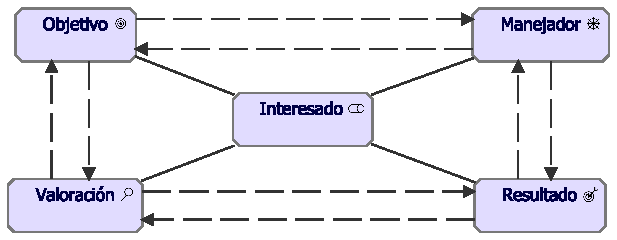
\includegraphics[width=1.0\linewidth]{imgs/modelo/Interesado}
	\caption{Modelo Implicados}
\end{figure}

Los elementos de motivación se utilizan para modelar las motivaciones, o razones, que guían el diseño o el cambio de una arquitectura empresarial, y es esencial comprender los factores, a menudo denominados impulsores, que influyen en otros elementos de motivación.  Pueden originarse tanto dentro como fuera de la empresa.  Los impulsores internos, también llamados preocupaciones, están asociados con las partes interesadas, que pueden ser algún ser humano individual o algún grupo de seres humanos, como un equipo de proyecto, una empresa o la sociedad. Ejemplos de esos impulsores internos son la satisfacción del cliente, el cumplimiento de la legislación o la rentabilidad. Es común que las empresas realicen una evaluación de esos factores impulsores; por ejemplo, utilizando un análisis FODA, a fin de responder de la mejor manera posible.

%\newpage

\subsection{Caso  de Implicados}
\begin{figure}[h!]
	\centering
	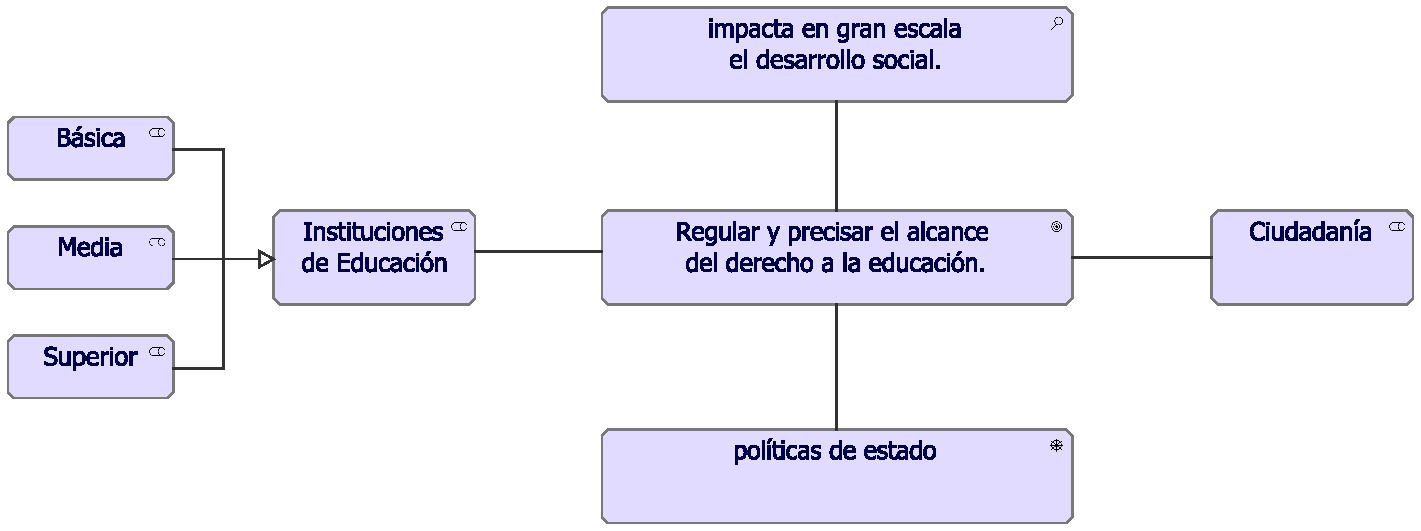
\includegraphics[width=1.0\linewidth]{imgs/motivacion/implicados/imp1.pdf}
	\caption{Caso Implicados}
\end{figure}

Los elementos, principalmente externos que se encuentran fuertemente ligados para regular y precisar el alcance del derecho a la educación, son las políticas de Estado vigentes y en desarrollo dispuestas por la administración a cargo. Por otra parte, la valoración comprendida en este objetivo, impacta en gran medida el desarrollo social del país, debido a que son ellos, la comunidad quienes dispondrán de la oportunidad educarse para forjar un mejor futuro tanto para sus familias como para la comunidad en general. Así mismo, las instituciones de educación básica, media y superior, quienes permiten y promueven la adquisición de habilidades, conocimientos y la ampliación de horizontes personales, a través de los lineamientos dispuestos por el MEN, son otro de los interesados alrededor de este objetivo.